%\documentclass[hyperref={colorlinks=true}]{beamer}
\documentclass[handout,hyperref={colorlinks=true}]{beamer}

\usepackage{pgfpages}
\pgfpagesuselayout{2 on 1}[a4paper,border shrink=5mm]
\usepackage[spanish]{babel}
\usepackage[utf8x]{inputenc}
\usepackage{times}
\usepackage[T1]{fontenc}
\usepackage{amssymb,amsmath}
\usepackage{enumerate}
\usepackage{verbatim}
%\usepackage{pst-all}
%\usepackage{pstricks-add}
\usepackage{array}
%\usepackage[T1]{fontenc}
\usepackage{animate,movie15}
%\usepackage{media9}
%% newcommand

\newcommand{\com}{\mathbb{C}}
\newcommand{\dis}{\mathbb{D}}
\newcommand{\rr}{\mathbb{R}}
\newcommand{\sen}{\hbox{sen }}
\newcommand{\oo}{\mathcal{O}}
\renewcommand{\emph}[1]{\textcolor[rgb]{1,0,0}{#1}}
\renewcommand{\epsilon}{\varepsilon}
\newcommand{\nl}{\onslide<+-> }


\newtheorem{teorema}{Teorema}[section]
\newtheorem{lema}[teorema]{Lema}
\newtheorem{corolario}[teorema]{Corolario}
\newtheorem{proposicion}[teorema]{Proposici\'on}
\newtheorem{definicion}[teorema]{Definici\'on}

\newenvironment{demo}{\noindent\emph{Dem.}}{$\square$ \newline\vspace{5pt}}


\mode<all>
{
  \usetheme{Boadilla}
  % oder ...
 
  \setbeamercovered{wolverine}
  % oder auch nicht
}




\usepackage{times}

\title[Introducción a las ecuaciones] % (optional, nur bei langen Titeln nötig)
{%
Introducción a las ecuaciones
}



\author[] % (optional, nur bei vielen Autoren)
{Fernando Mazzone}

\institute[Depto de Matemática] % (optional, aber oft nötig)
{
 Depto de Matemática\\
Facultad de Ciencias Exactas Físico-Químicas y Naturales\\
Universidad Nacional de Río Cuarto}


\subject{Ecuaciones Diferenciales}

\begin{document}

\begin{frame}
  \maketitle
  \begin{center}
   
\includegraphics[scale=0.2]{imagenes/unrc.jpg}
   \end{center}
\end{frame}















\section{Sobre esta materia}

\begin{frame}{Sobre la materia}

\begin{itemize}
 \item  \href{https://docs.google.com/viewer?a=v&pid=sites&srcid=ZGVmYXVsdGRvbWFpbnxlY3VhY2lvbmVzZGlmZXJlbmNpYWxldW5yY3xneDoyZjE0YzJmMDcyODc0ZGQ3}{Programa analítico.}
 \item  \href{https://sites.google.com/site/ecuacionesdiferencialeunrc/ecuaciones-diferenciales-unrc}{Página web} de la materia
 \item  Vamos a hacer uso intensivo de \href{http://www.sagemath.org/}{SAGE}.
 \item  Requeriremos muchos contenidos de la asignatura Física.
 \item  \begin{tabular}{m{4cm} m{2cm}} Bibliografía principal & 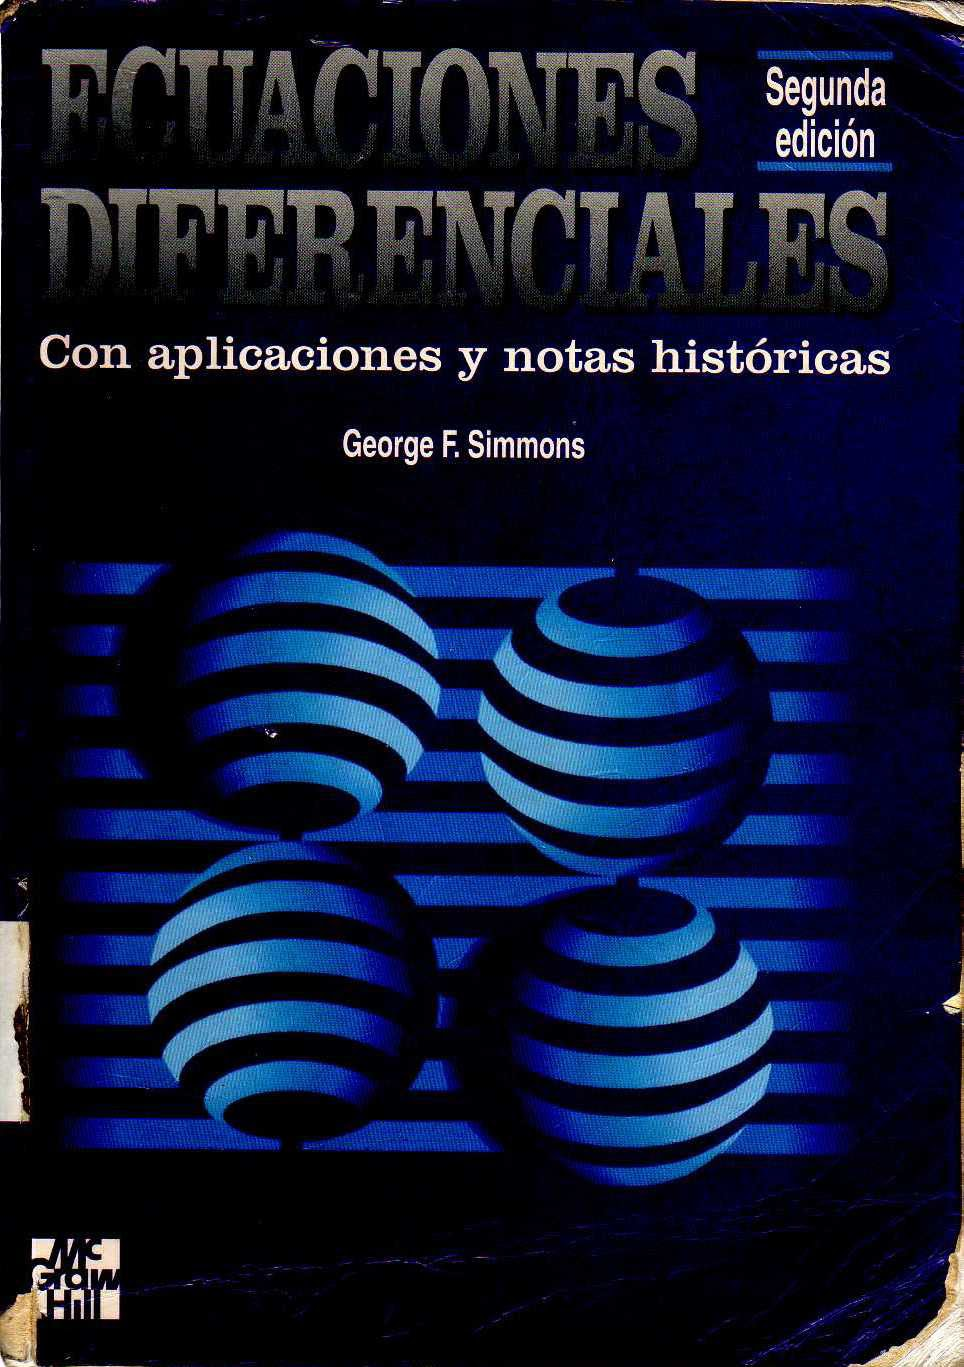
\includegraphics[scale=0.05]{imagenes/Tapa_Simmons.jpg}           \end{tabular} 

\end{itemize}

\end{frame}

\section{¿Que son las ecuaciones diferenciales?}
\begin{frame}{¿Que son las ecuaciones diferenciales?}

\begin{block}{Ecuación diferencial, definición informal}
 Es una o varias relaciones entre una o varias variables dependientes y sus tasas de cambio respecto a ciertas variables independientes. El problema básico asociado
 a las ecuaciones es hallar las variables dependientes que las resuelven. Las ecuaciones diferenciales son usadas muy a menudo en matemática aplicada, puesto que muchas 
 leyes (de la física por ejemplo) justamente establecen este tipo de ecuaciones. 
\end{block}



\end{frame}


\begin{frame}{Caída libre}

\nl \textbf{Ejemplo, \href{http://es.wikipedia.org/wiki/Caída_libre}{caída libre}} Modelizar matemáticamente el movimiento de un cuerpo de masa $m$ en las proximidades de la superficie
terrestre, asumiendo que su movimiento es
sobre la vertical y que las fuerzas que sobre él actúan son la gravedad y el rozamiento con el aire.

\nl \begin{tabular}{m{4.5cm} m{5cm}} 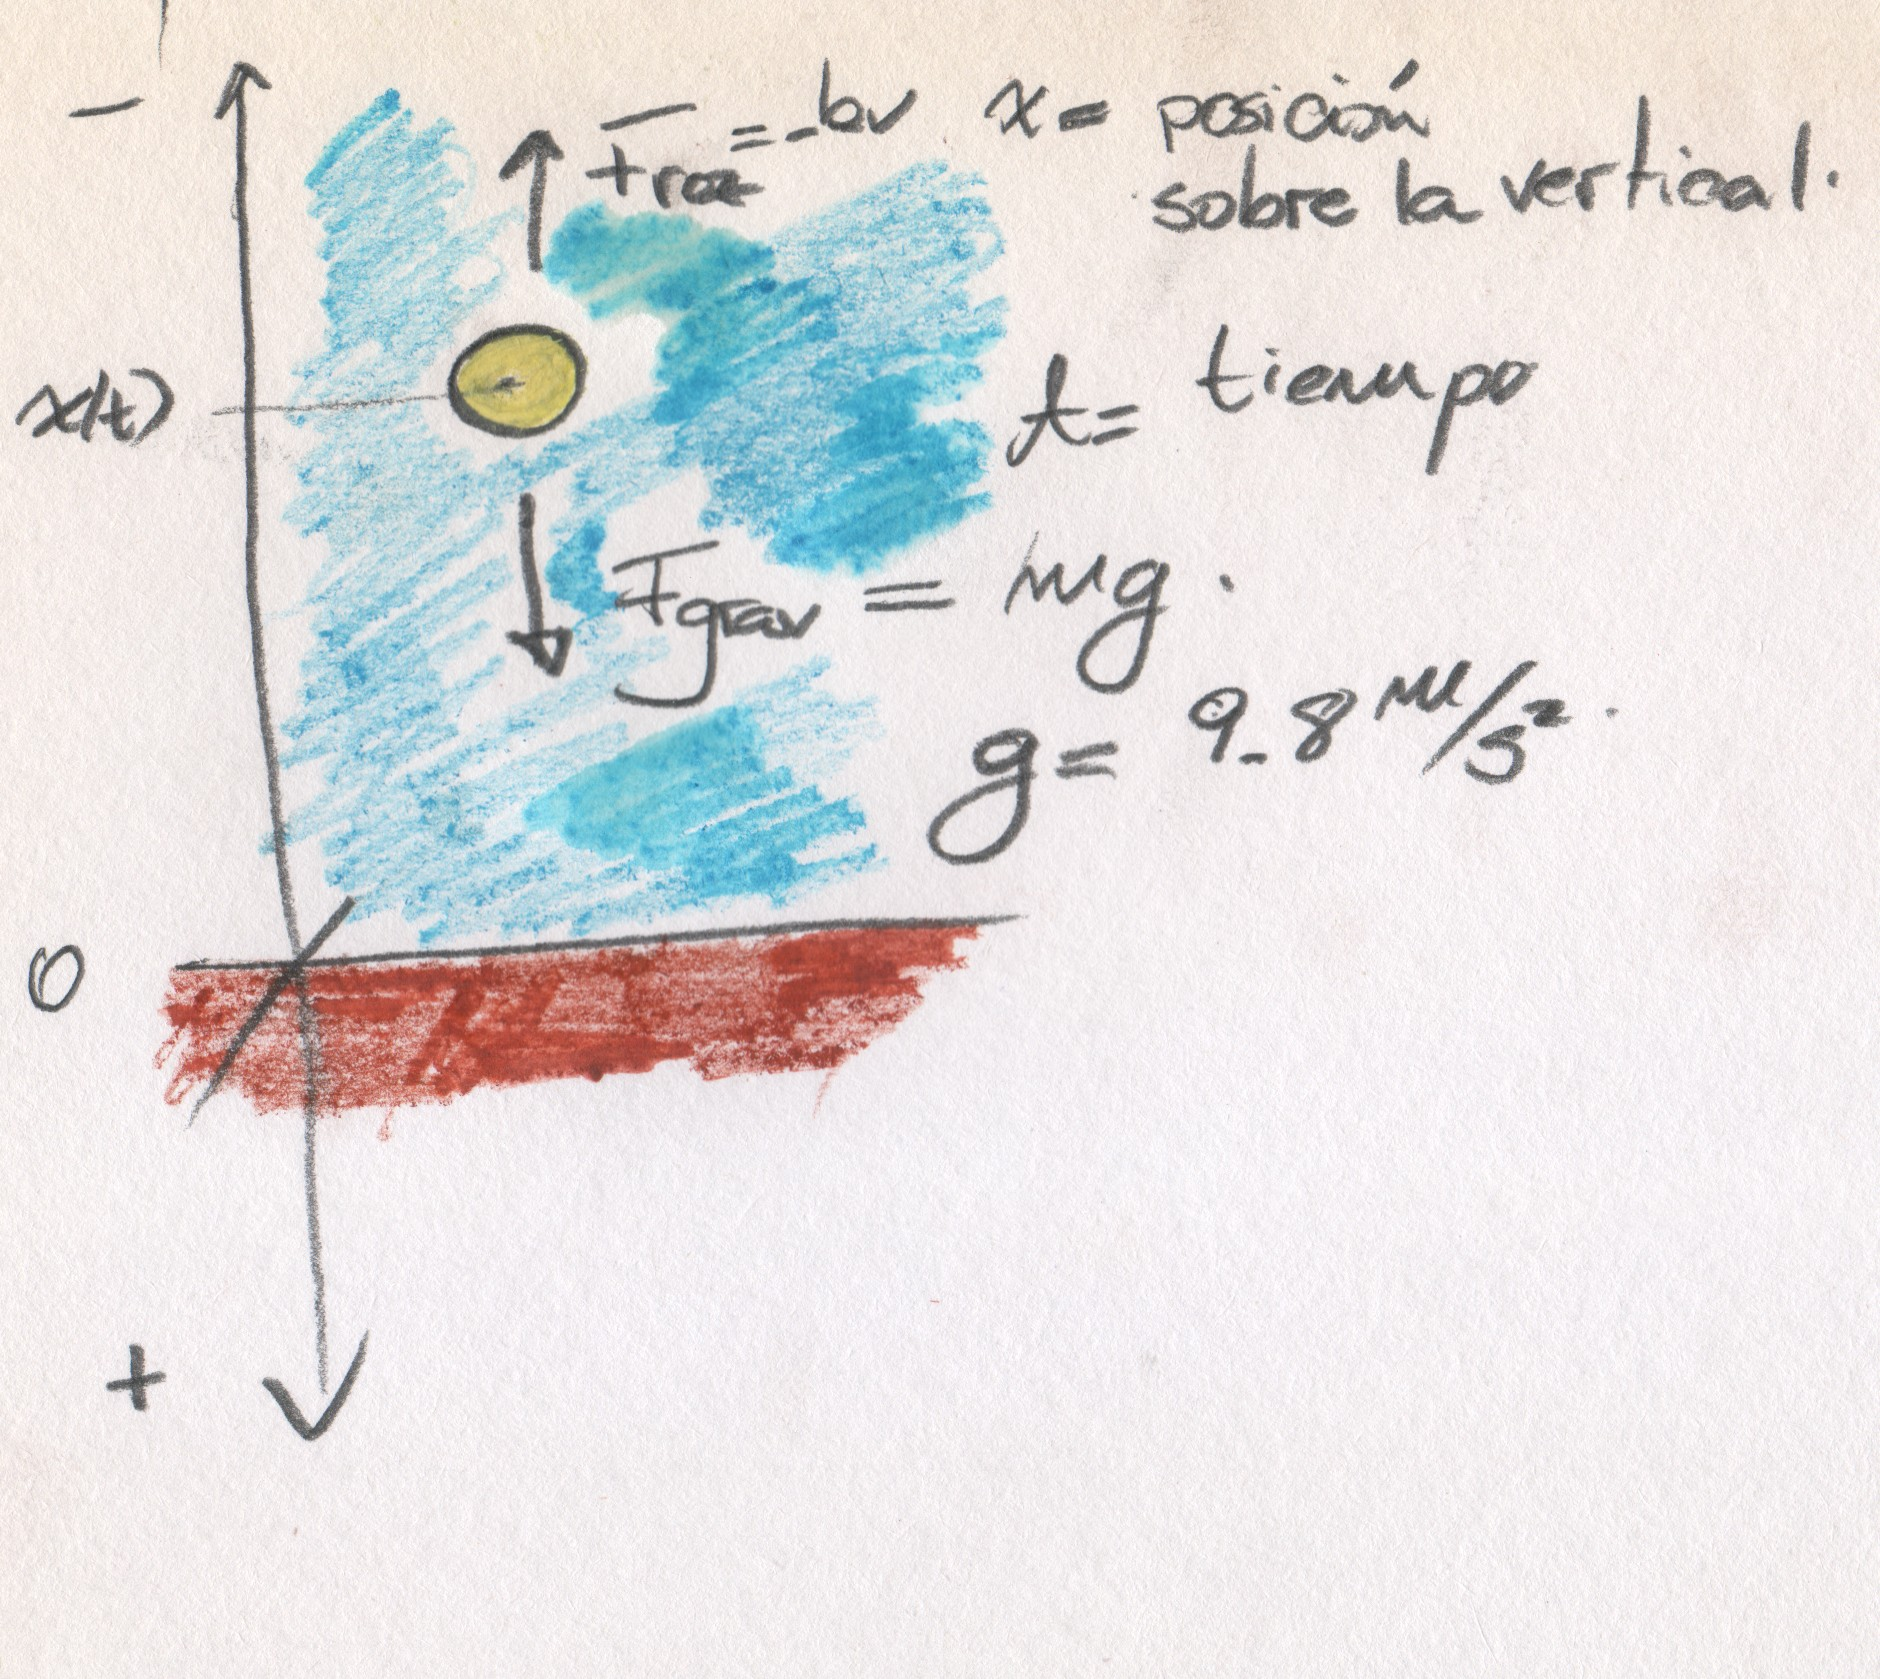
\includegraphics[scale=0.07]{imagenes/caida_libre.jpg}    &  $x(t)=$ posición a lo largo de la vertical, relativo a un eje de coordenadas\newline
$v(t)=\frac{dx}{dt}=$ velocidad\newline
$F_{grav}=$ fuerza debida a la gravedad $=mg$ donde $g=9.8m/s^2$
$F_{roz}=$ fuerza de rozamiento, proporcional a la velocidad y de sentido contrario $=-cv$, $c>0$.

\end{tabular} 
\end{frame}
\begin{frame}{Caída libre}

\nl Usamos la \href{http://es.wikipedia.org/wiki/Leyes_de_Newton}{Segunda Ley de Newton}, esto es la suma de las fuerzas totales que actuan sobre un cuerpo de masa $m$
es igual al producto de la masa $m$ y la aceleración $a(t)$. Recordemos que la aceleración es la tasa de cambio de la velocidad, es decir la derivada segunda de la posición.   

\nl  Usando todas las relaciones mencionadas

\[ma(t)=mv'(t)=F_{\hbox{total}}=F_{\hbox{grav}}+F_{\hbox{roz}}=mg-cv\]

vale decir
\begin{equation}\label{caidaLibre1}
 \boxed{ x''(t)+\frac{c}{m} x'(t)=g.}
\end{equation}
\begin{equation}\label{caidaLibre2}
\boxed{ v'(t)+\frac{c}{m} v=g.}
\end{equation}
\end{frame}



\begin{frame}{Algunos conceptos relacionados con ecuaciones diferenciales}
\begin{itemize}
\nl  \item \textbf{Orden} El índice de la mayor derivada interviniente en la ecuación. Por ejemplo la ecuación \eqref{caidaLibre1} es de orden 2 y la
ecuación \eqref{caidaLibre2}, si bien está estrechamente relacionada con la anterior, es de orden 1. Como regla casi general, conviene tener menor orden.

\nl  \item \textbf{Solución} Una función que satisface la relación que indica la ecuación. Por ejemplo
\begin{equation}\label{SolGencaidaLibre2} v(t)=\frac{m}{c}g+ke^{-\frac{c}{m}t},\end{equation}
resuelve \eqref{caidaLibre2}, para todo $C\in\rr$. No deberíamos perder tiempo en chequear una cuestión tan sencilla, pero aprovechemos la ocasión para presentar 
un recurso que utilizaremos de manera sistemática: \href{https://sage.ccad.unrc.edu.ar/home/pub/63/}{SAGE}.

\end{itemize}

 

\end{frame}

\begin{frame}{Algunos conceptos relacionados con ecuaciones diferenciales}
\begin{itemize}
\nl  \item \textbf{Ecuación diferencial ordinaria} Es una ecuación donde las variables dependientes sólo dependen de una única variable independiente. Las 
ecuaciones \eqref{caidaLibre1} y \eqref{caidaLibre2} son ejemplo de ello, la variable independiente es el tiempo.
\nl  \item \textbf{Ecuación en derivadas parciales} Es una ecuación donde las variables dependientes dependen de más de una variable independiente. 
Ejemplo de este tipo de ecuación es la ecuación de Laplace

\[\frac{\partial^2 u}{\partial x^2}+\frac{\partial^2 u}{\partial y^2}=0\]

\end{itemize}
\end{frame}

\begin{frame}{Algunos conceptos relacionados con ecuaciones diferenciales}
\begin{itemize}
\nl  \item \textbf{Sistema de ecuaciones} También puede ocurrir  que tengamos varias variables dependientes. En ese caso tendríamos varias incognitas en 
nuestro problema. En general una sóla ecuación no sirve para determinar todas las incognitas, sino que, a semejanza de lo que ocurre con ecuaciones algebraicas, es 
necesario tener tantas ecuaciones como incognitas. En ese caso hablamos de sistema de ecuaciones. Por ejemplo, el sistema de ecuaciones para el resorte

\[\left\{ \begin{array}{l l} x'&=y \\y'&=-\sen(x) \end{array}\right.\]


\end{itemize}

 

\end{frame}


\begin{frame}{Algunos conceptos relacionados con ecuaciones diferenciales}
 
\nl  \textbf{Resolver una ecuación} Muy a menudo hablaremos de resolver una ecuación, pero es oportuno discutir que queremos significar con esto.  
Por resolver entenderemos expresar la solución como combinaciones algebraicas y composiciones de funciones que consideramos elementales, por ejemplo potencias, exponenciales, logarítmos, trigonométricas
y trigonométricas inversas. El universo de funciones que se considera elemental es una cuestión de gusto. Las operaciones permitidas para combinar estas funciones
también. Por ejemplo, admitiremos como válida una expresión que contenga una integral, al menos en el caso que no sea claro como resolver esta integral.

\nl Casi todo este curso trata con la discusión de métodos para resolver ecuaciones.
 

\end{frame}


\begin{frame}{Algunos conceptos relacionados con ecuaciones diferenciales}
 
\nl  \textbf{Solución general} Comunmente una ecuación presenta infinitas soluciones. Una solución general  es una expresión para las soluciones que 
contiene parámetros. Cada elección de estos parámetros determina una solución distinta. Por ejemplo \eqref{SolGencaidaLibre2} es la solución general de \eqref{caidaLibre2}.

\nl  La afirmación anterior requiere una demostración puesto que sólo hemos mostrado que \eqref{SolGencaidaLibre2} es solución, pero no
que toda solución se expresa con \eqref{SolGencaidaLibre2}. Para demostrar la afirmación, hay que multiplicar ambos miembros de \eqref{SolGencaidaLibre2} 
por $e^{\frac{c}{m}t}$ y luego intergar respecto a $t$ 
\[\frac{mg}{c}e^{\frac{c}{m}t}=\int ge^{\frac{c}{m}t}dt=\int \left(v'(t)e^{\frac{c}{m}t}+\frac{c}{m}e^{\frac{c}{m}t}\right) vdt=e^{\frac{c}{m}t}v+C.\]
 Despejando $v$ del primer y último miembro obtenemos \eqref{SolGencaidaLibre2} con $k=-C$.

 

\end{frame}

\begin{frame}{Algunos conceptos relacionados con ecuaciones diferenciales}
\textbf{Ejemplo} En algunas ocasiones sólo podemos dejar una relación implícita entre las variable dependientes e independientes. Por ejemplo
\begin{equation}\label{solImpl}x=e^y+y+C\quad\text{ para } C\in\rr\end{equation}
es solución general de
\[y'(e^y+1)=1.\]
Vamos a chequear sólo que \eqref{solImpl} es solución, dejando la justificación que toda solución tiene esa forma para más adelante. Derivando \eqref{solImpl}
\[ 1=e^yy'+y'\]
Luego $y'=1/(1+e^{y})$. Reemplazando esta relación  en la ecuación diferencial corroboramos que es solución.

\end{frame}

\section{Definición formal}
\begin{frame}{Definición formal}
\begin{block}{Ecuación diferencial} Una ecuación diferencial ordinaria de orden $n$ es una relación de la forma
\[\boxed{F(x,y(x),y'(x),\ldots,y^{(n)}(x))=0}.\]
donde
\[F:(a,b)\times \Omega\to\rr,
\]
donde $\Omega$ es abierto de $\rr^{n+1}$ y $(a,b)$ un intervalo de $\rr$.
 
\end{block}


\end{frame}

\begin{frame}{Primitivas y ecuaciones}
\textbf{Ejemplo} El problema de hallar una primitiva de una función es una ecuación diferencial que, como ya haz visto en curso iniciales de análisis, se resuelve 
con la integral. Supongamos $f:(a,b)\subset \rr\to\rr$ una función continua. Consideremos la ecuación diferencial
\[y'(x)=f(x).\]
Sea $x_0\in(a,b)$, integrando respecto a $x$ entre $x_0$ y $x$
\[y(x)=y(x_0)+\int_{x_0}^xf(t)dt\]
Que es una solución general. Quedaría determinada una única solución si, por ejemplo, conociecemos $y(x_0)$.
\end{frame}

\begin{frame}{Primitivas y ecuaciones}
\textbf{Ejemplo} Supongamos $f:(a,b)\subset \rr\to\rr$ como antes. Consideremos la ecuación diferencial
\[y''(x)=f(x).\]
Tomemos una integral indefinida respecto a $x$ 
\[y'(x)=C_1+\int f(t)dt\]
Ahora deberemos tomar una integral indefinida más
\[y(x)=C_2+C_1t +\int\left(\int f(x)dx\right)dx.\]
Ahora quedan dos constantes $C_1$ y $C_2$. 
\end{frame}


\begin{frame}{Principio de Hadamard}
\nl \begin{block}{Principio de Hadamard}
 Un problema se dice \href{http://es.wikipedia.org/wiki/Problema_bien_definido}{bien planteado} segun Hadamard si satisface que
 \begin{enumerate}
  \item El problema admite solución
  \item La solución es única
  \item La solución depende de manera continua de los datos numéricos del problema.
 \end{enumerate}
 \end{block}
\nl Como hemos visto, una ecuación diferencial no determina una única solución, por consiguiente no sería un problema bien planteado. Debemos agregar relaciones
a nuestro problema para que sea bien planteado. Es así que aparecen condiciones iniciales, problemas de contorno, etc.
 


\end{frame}


\begin{frame}{Problemas de valores iniciales}
\begin{block}{Problemas de valores iniciales} Sea $x_0\in(a,b)$, $F:(a,b)\times \Omega\to\rr$ e $y_0,y_0^1,\ldots,y_0^{n-1}\in\rr$. Las siguientes relaciones  se denominan problemas de 
valores iniciales
\[
 \left\{\begin{array}{l l l}
         F(x,y,y',&\ldots,y^{(n)})=0& x\in(a,b)\\
         y(x_0)&=y_0&\\
         y'(x_0)&=y_0^1&\\
          & \vdots &\\
          y^{(n-1)}(x_0)&=y_0^{n-1}&\\
        \end{array}
   \right.
\]
\end{block}
\end{frame}


\begin{frame}{Ecuaciones de primer orden}
\begin{block}{Ecuaciones de primer orden} La ecuación general de primer orden tiene la forma
\[
F(x,y(x),y'(x))=0,
\]
donde $F:(a,b)\times \Omega\to\rr$, $\Omega$ abierto de $\rr^2$. Con frecuencia asumiremos que $y'$ se despeja de la relación anterior, es decir que existe $f:\Omega'\to\rr$,
$\Omega'$ abierto de $\rr^2$, tal que
\[y'=f(x,y).\]
Bajo esta suposición, si $(x_0,y_0)\in\Omega'$ el problema de valores iniciales se escribe
\[\left\{\begin{array}{l l}
	    y'&=f(x,y)\\
	    y(x_0)&=y_0
         \end{array}\right.
\]
\end{block}
\end{frame}


\section{Famílias paramétricas de funciones}

\begin{frame}{Familias paramétricas de funciones} 

\begin{block}{Problema}
 Dada una familia paramétrica de funciones
 \begin{equation}\label{flia_param}y=y(x,c),\end{equation}
 dependiente del parámetro $c\in\rr$, ¿Será posible hallar una ecuación para la cual la familia sea la solución general?
\end{block}
  
\end{frame}

\begin{frame}{Familias paramétricas de funciones} 
En líneas generales la respuesta es si. Nos conviene expresar \eqref{flia_param} como una ecuación implícita
\begin{equation}\label{flia_impl}f(x,y,c)=0.\end{equation}
Derivando esta ecuación respecto a $x$
\begin{equation}\label{der_impl}
 \frac{\partial f}{\partial x}+\frac{\partial f}{\partial y}y'(x,c)=0.
\end{equation}
Ahora es posible eliminar $c$ de \eqref{flia_impl} y \eqref{der_impl} al costo de quedarnos con una sola ecuación.

\end{frame}

\begin{frame}{Familias paramétricas de funciones} 
\textbf{Ejemplo 1} Encontrar la ecuación que satisface la familia paramétrica
\[x^2+y^2=c^2.\]
Derivamos
\[2x+2yy'=0.\]
Ya está!!!

\textbf{Ejemplo 2} Idem $x^2+y^2=2cx$.  Derivando
\[2x+2yy'=2c.\]
Eliminamos $c$ de las dos relaciones
\[\frac{x^2+y^2}{x}=2x+2yy'\Rightarrow \boxed{y'=\frac{y^2-x^2}{2xy}}.\]

\end{frame}

\begin{frame}{Familias paramétricas de funciones} 
\begin{block}{Problema}
 Dada una familia paramétrica
 \[f(x,y,c)=0,\]
 encontrar otra
 \[g(x,y,d)=0\]
 tal que cada punto de corte del gráfico de las funciones de una y otra familia sea en ángulos rectos. 
\end{block}


\end{frame}

\begin{frame}{Familias paramétricas de funciones} 
Para resolver este problema se completan estos pasos
\begin{itemize}
 \item Se encuentra la ecuación diferencial que satisface la familia dada, digamos
 \[y'=h(x,y).\]
 \item Se resuelve
 \[y'=-\frac{1}{h(x,y)}.\]
\end{itemize}



\end{frame}

\begin{frame}{Familias paramétricas de funciones} 
 \textbf{Problema}: encontrar la familia de curvas ortogonales a la flia de circunferencias

\[x^2+y^2=c^2\]

Solución: ver la \href{https://sage.ccad.unrc.edu.ar/home/pub/63/}{notebook de SAGE}
\end{frame}

\section{Separación de variables}
\begin{frame}{Separación de variables}
\begin{block}{Ecuaciones en variables separadas} Se dice que en una ecuación de primer orden
 \[y'=f(x,y)\]
 separan las variables, si es posible la factorización $f(x,y)=g(x)h(y)$.
 \end{block}



\end{frame}

\begin{frame}{Separación de variables} 
Una ecuación  en la que se separan variables se puede resolver siguiendo los siguientes pasos. Como
\[\frac{y'}{h(y)}=g(x),\]
Si $H$ y $G$ son primitivas de $1/h$ y $g$ respectivamente por la regla de la cadena tenemos
\[\frac{d}{dx}H(y)=\frac{d}{dx}G(x)\]
Luego 
\[H(y)=G(x)+C,\quad C\in\rr.\]
Si podemos encontrar la inversa de $H$
\[y(x)=H^{-1}\left(G(x)+C\right).\]


\end{frame}

\begin{frame}{Separación de variables} 
\textbf{Ejemplo:} Resolver
\[y'=\frac{y}{x}.\]
Es común emplear el método de la siguiente forma
\[\begin{split}
   \frac{dy}{dx}=\frac{y}{x} &\Longrightarrow \frac{dy}{y}=\frac{dx}{x} \Longrightarrow \int \frac{dy}{y}=\int \frac{dx}{x}\\
   &\Longrightarrow\ln|y|=\ln|x|+C \Longrightarrow |y|= k|x|, \hbox{ con }k>0\\
   &\Longrightarrow y= kx, \hbox{ con }k\in\rr
  \end{split}
\]

\end{frame}

\section{Galeria de Ejemplos}

\begin{frame}{Ley de reproducción normal}
\nl  En muchos ejemplos de bilogía, química-física, etc, hay magnitudes que crecen(decrecen) siguiendo una ley que denominaremos 
\href{http://es.wikipedia.org/wiki/Crecimiento_exponencial}{Ley de reproducción  normal}. Según esta ley la cantidad de individuos, sustancia, materia,
energía, etc, que se agrega o elimina de una población, cuerpo, etc por unidad de tiempo es proporcional a la cantidad de individuos, sustancia, etc que hay presente.

\end{frame}

\begin{frame}{Ley de reproducción normal}
\nl  Una población de seres vivos puede reproducirse de esta manera bajo algunas circunstancias 
especiales, por ejemplo si cuenta con fuente ilimitada de alimentos.

\nl  Si $P(t)$ es la cantidad de individuos en el momento $t$, la ley de reproducción normal establece
en este caso la siguiente ecuación diferencial de primer orden
\[P'(t)=kP(t),\quad\text{ con } k>0.\]
La solución es hallada con suma facilidad, siendo ella 
\[\boxed{P(t)=Ce^{kt},\quad C\in\rr.}\]
La constante  $C$ se puede determinar si tenemos un problema a valores iniciales (pvi), por ejemplo $P(0)=P_0$, siendo $P_0\in\rr$ dado. En ese caso
$A=P_0$. 
\end{frame}

\begin{frame}{Decaimiento radioactivo}
\nl  Otro ejemplo de comportamiento similar es la \href{http://es.wikipedia.org/wiki/Radiactividad}{desintegración radiactiva}. Algunos átomos de
ciertas sustancias, pueden ``desarmarse'' en átomos de otras sustancias. En el proceso suelen emitir radiaciones.  La velocidad de desintegración sigue una ley
de reproducción normal pero hay que tener en cuenta que la materia en este caso se pierde. Si $x(t)$ es la masa de materia radiactiva en el momento $t$, evolucionará 
acorde a la ley
\[\boxed{x'(t)=-kx(t),\quad\text{con } k>0.}\]

\end{frame}

\begin{frame}{Soluciones}
\begin{tabular}{m{5cm} m{4.5cm}}
 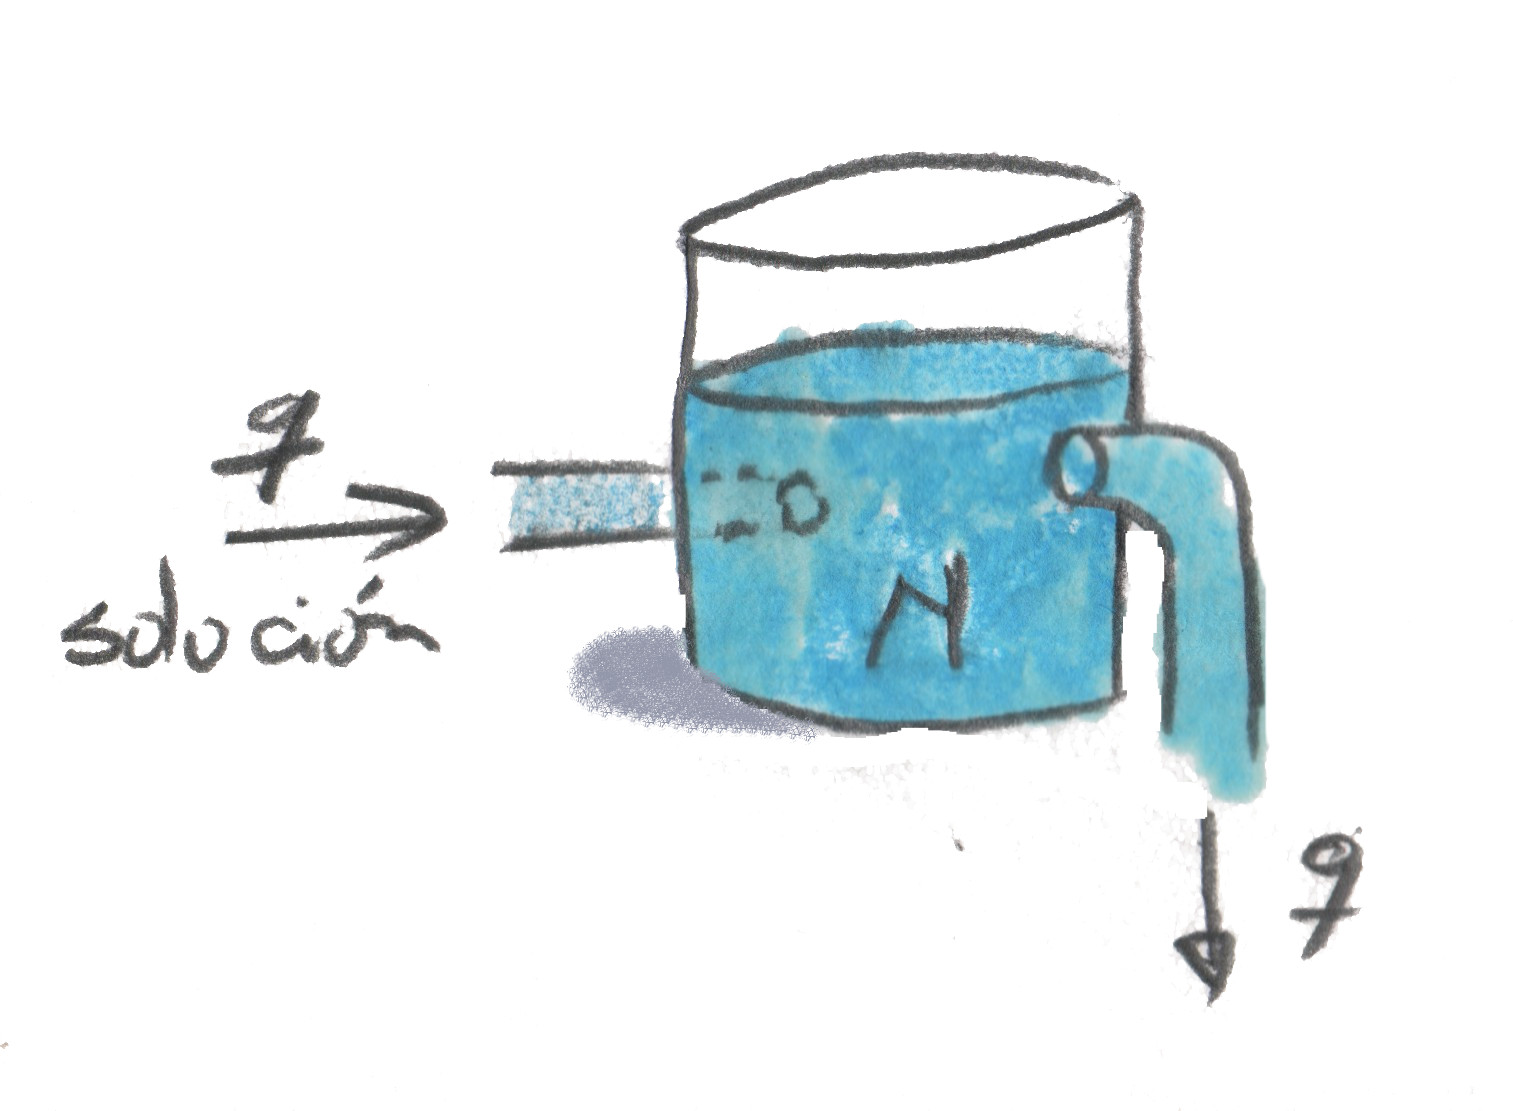
\includegraphics[scale=.1]{imagenes/tanque.jpg} & Un tanque contiene inicialmente $N$ $\hbox{m}^3$ de $H_2O$ entre los cuales hay disueltos $C$ kg de sal común
 $NaCl$. A través de una boca de entrada y una de salida empieza circular la solución, entrando y saliendo al mismo caudal $q\frac{\hbox{m}^3}{s}$. Se supone que 
 la solución entrante tiene una concentración conocida $r$. Encontrar la cantidad de sal en el momento $t$. \\
\end{tabular}


\end{frame}


\begin{frame}{Soluciones}
\textbf{Solución} Sea $x(t)$ la cantidad de $NaCl$ en el tanque en el momento $t$. entonces

\[\begin{split}
   x'(t)&=\text{cantidad que entra }-\text{cantidad que sale }\\
          &=qr-q\frac{x(t)}{N}
  \end{split}
\]


\end{frame}

\begin{frame}{Dinámica del punto}
Vamos a recordar algunas temas de la asignatura física. En particular  el movimiento de un cuerpo de masa $m$ al que podemos suponer puntual. Lo llamaremos punto masa. Denotamos por $x(t)$ su posición, digamos en $\rr^3$. Y suponemos 
que sobre él actúa una fuerza $f$. Recordemos que $x'(t)$ es la velocidad $v(t)$ y que $x''(t)$ es la aceleración $a(t)$.  
\href{http://es.wikipedia.org/wiki/Leyes_de_Newton\#Segunda_ley_de_Newton_o_ley_de_fuerza}{La segunda ley de Newton} implica que 
\begin{equation}\label{2leyR}\boxed{mx''(t)=f}\end{equation}



\end{frame}

\begin{frame}{Dinámica del punto}

Supongamos que el movimiento del punto masa se realiza entre los momentos $t_0$ y $t_1$. Como has visto en Cálculo III la lóngitud de la curva recorrida 
$s(t)$ se puede calcular por
\begin{equation}\label{2ley}s=\int_{t_0}^{t_1}|x'(t)|dt=\int_{t_0}^{t_1}|v(t)|dt.\end{equation}
A $s$ se lo suele denominar \href{http://es.wikipedia.org/wiki/Longitud_de_arco}{elemento de arco}. Es comun querer utilizar a $s$ como variable independiente en 
lugar de $t$, puesto que algunas fórmulas se simplifican si se lo utiliza. Por ejemplo

\begin{equation}\label{pre_trab} f\cdot v(t)dt=f\cdot\frac{v(t)}{|v(t)|}|v(t)|dt=f_tds,\end{equation}
donde $f_t$ denota la proyección de la fuerza $f$ sobre la dirección tangente a la trayectoria.




\end{frame}

\begin{frame}{Dinámica del punto}
Si integramos \eqref{pre_trab} entre $t_0$ y $t_1$ y usamos \eqref{2leyR} obtenemos
\[\begin{split} W:=\int_{s_0}^{s_1}f_tds&=\int_{t_0}^{t_1} f\cdot v(t)dt\\
   & =m \int_{t_0}^{t_1} v'(t)\cdot v(t)dt\\
   &=\frac{m}{2} \int_{t_0}^{t_1} \frac{d|v|^2}{dt}dt\\
   &=\frac{m}{2}|v(t_1)|^2-\frac{m}{2}|v(t_0)|^2.  \end{split}\]
\end{frame}


\begin{frame}{Dinámica del punto}
\nl  A la cantidad $\frac{m}{2}|v|^2$ se la denomina energía cinética $E_c$ y a $W$ se lo denomina trabajo. 
Las relaciones obtenidas dicen que la variación de la energía cinética es igual al trabajo realizado $W=\Delta E_c$. 
El trabajo realizado depende de la proyección tangencial de la fuerza $f_t$.  Llamaremos a esta relación
Principio de Conservación de la Energía Mecánica.

\nl  Vamos a referirnos por rapidez al módulo de la velocidad. 
Si uno quiere incrementar o reducir la rapidez final $|v(t_1)|$ entonces deberá tener fuerzas con una componente tangencial no nula. 
Dicho de otra forma, si la fuerza es perpendicilar al movimiento, no hay cambio de rapidéz. 

\nl  Hay fuerzas que siempre actuan en la dirección del movimiento. El ejemplo más conocido son las fuerzas de fricción, resistencia del aire,
resistencia a la rodadura, etc. Estás fuerzas, actúan sólo en la dirección del movimiento y se oponen a él.

\end{frame}

\begin{frame}{Dinámica del punto}
 

\nl  Por el contrario hay otras que actúan perpendiculares al movimiento $f_t=0$. Ejemplo de ello son las fuerzas que mantienen a un cuerpo moviéndosé a lo largo 
de una guía. Por ejemplo un niño cayendo por un tobogan. Que el niño no se despegue de la guía (tobogán) se explica por la aparición de una fuerza que se denomina
reacción de vínculo que actúa en la dirección perpendicular al movimiento esto es decir a la guía. Está fuerza debe compensar a toda otra fuerza que trata de apartar
al cuerpo de la guía.  En el caso del tobogán la gravedad trata de apartar al niño de él.


\end{frame}

\begin{frame}{Caída a lo largo de guías}

Analicemos más en detalle el movimiento de un cuerpo cayendo a lo largo de una guía estando además influído  por la acción de la gravedad. Supondremos el movimiento
en las proximidades de la superficie de la Tierra y por ello, supondremoa la fuerza de la gravedad constante $mg$. 
\begin{tabular}{m{5cm} m{4.5cm}}
 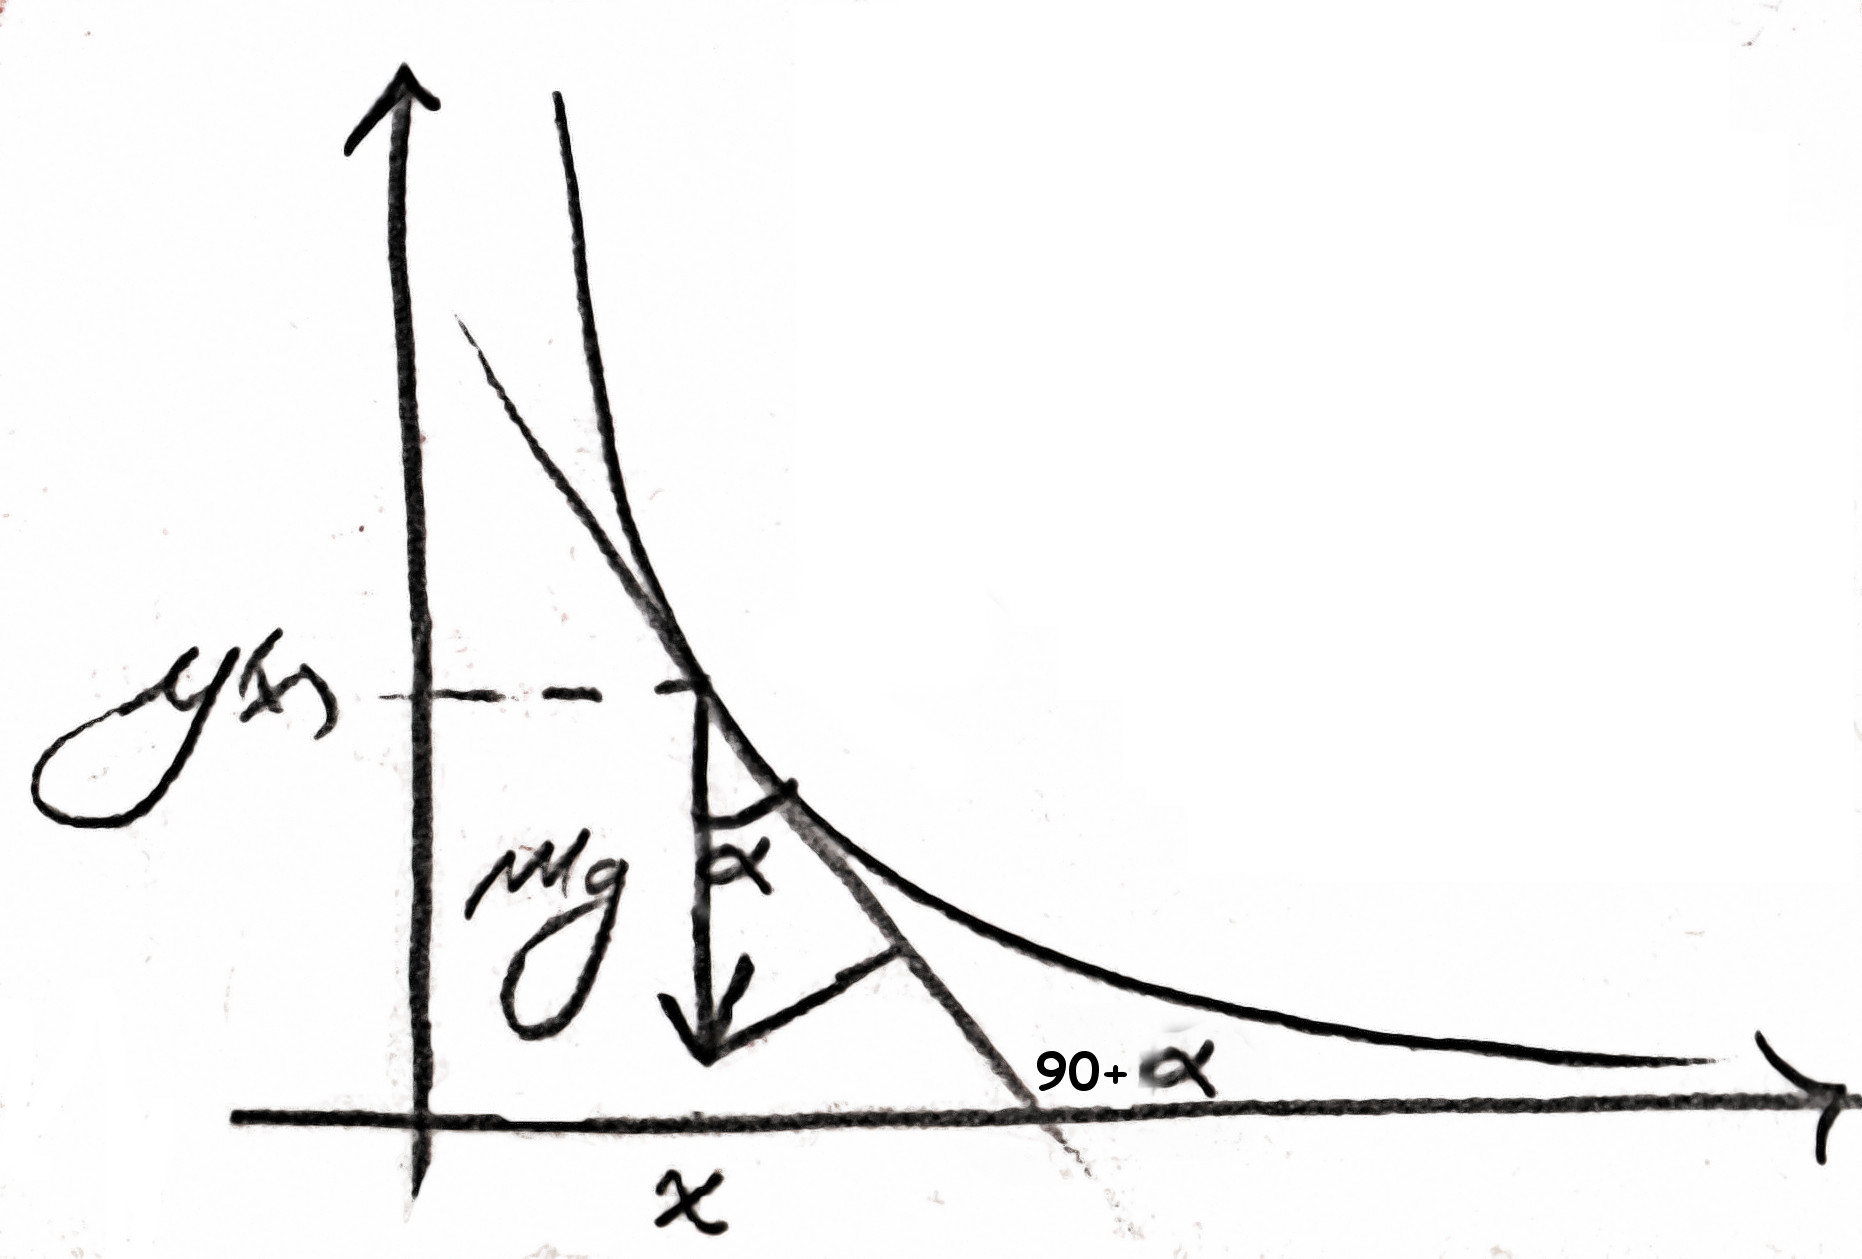
\includegraphics[scale=.07]{imagenes/caida_guia.jpg} & Supongamos que la guía esta
confinada a un plano. Introducimos un sistema de coordenadas ortogonales en dicho plano, con el suelo paralelo al eje $x$
\end{tabular}



\end{frame}


\begin{frame}{Caída a lo largo de guías}
El elemento longitud de arco $s$ de una curva que es el gráfico de una función $y(x)$ para $x$ en $[x_0,x_1]$ viene dado por 
\[s=\int_{x_0}^{x_1}\sqrt{1+y'(x)^2}dx\]
La fuerza de vínculo de la guía tiene componente tangencial nula,  la gravedad tiene una componente tangencial no nula. 
Su magnitud es $mg\cos\alpha$ (ver dibujo). Vamos a tratar de expresar $\cos\alpha$  en términos de   $y'(x)$. Vamos a suponer $\cos\alpha>0$ e $y'(x)<0$. 
Los demás casos quedan como \textbf{ejercicio}.
\[ \tan^2\alpha=\frac{\sen^2\alpha}{\cos^2\alpha}=\frac{1-\cos^2\alpha}{\cos^2\alpha}=\frac{1}{\cos^2\alpha}-1\]
y
\[y'(x)=\tan \left(\frac{\pi}{2}+\alpha\right)=-\frac{1}{\tan\alpha}\]

 

\end{frame}


\begin{frame}{Caída a lo largo de guías}
Podemos usar las relaciones anteriores para escribir $\cos\alpha$ en función de $y'(x)$
\begin{equation}\label{cos_alpha}\cos\alpha=-\frac{y'(x)}{\sqrt{1+y'(x)^2}}\end{equation}
Entonces
\begin{equation}\label{cons_ener}
 \begin{split} \frac{m}{2}|v(t_1)|^2-\frac{m}{2}|v(t_0)|^2&=\int_{s_0}^{s_1}f_tds =\int_{x_0}^{x_1}f_t\frac{ds}{dx}dx\\
&= -mg\int_{x_0}^{x_1}\frac{y'(x)}{\sqrt{1+y'(x)^2}}\sqrt{1+y'(x)^2}dx\\
&=-mg\left(y_1-y_0\right)
    \end{split}\end{equation}
Esto nos permite escribir la rapidez en función de la altura repecto al piso.
\end{frame}



\begin{frame}{El péndulo}
\begin{tabular}{m{4cm} m{5.5cm}}
 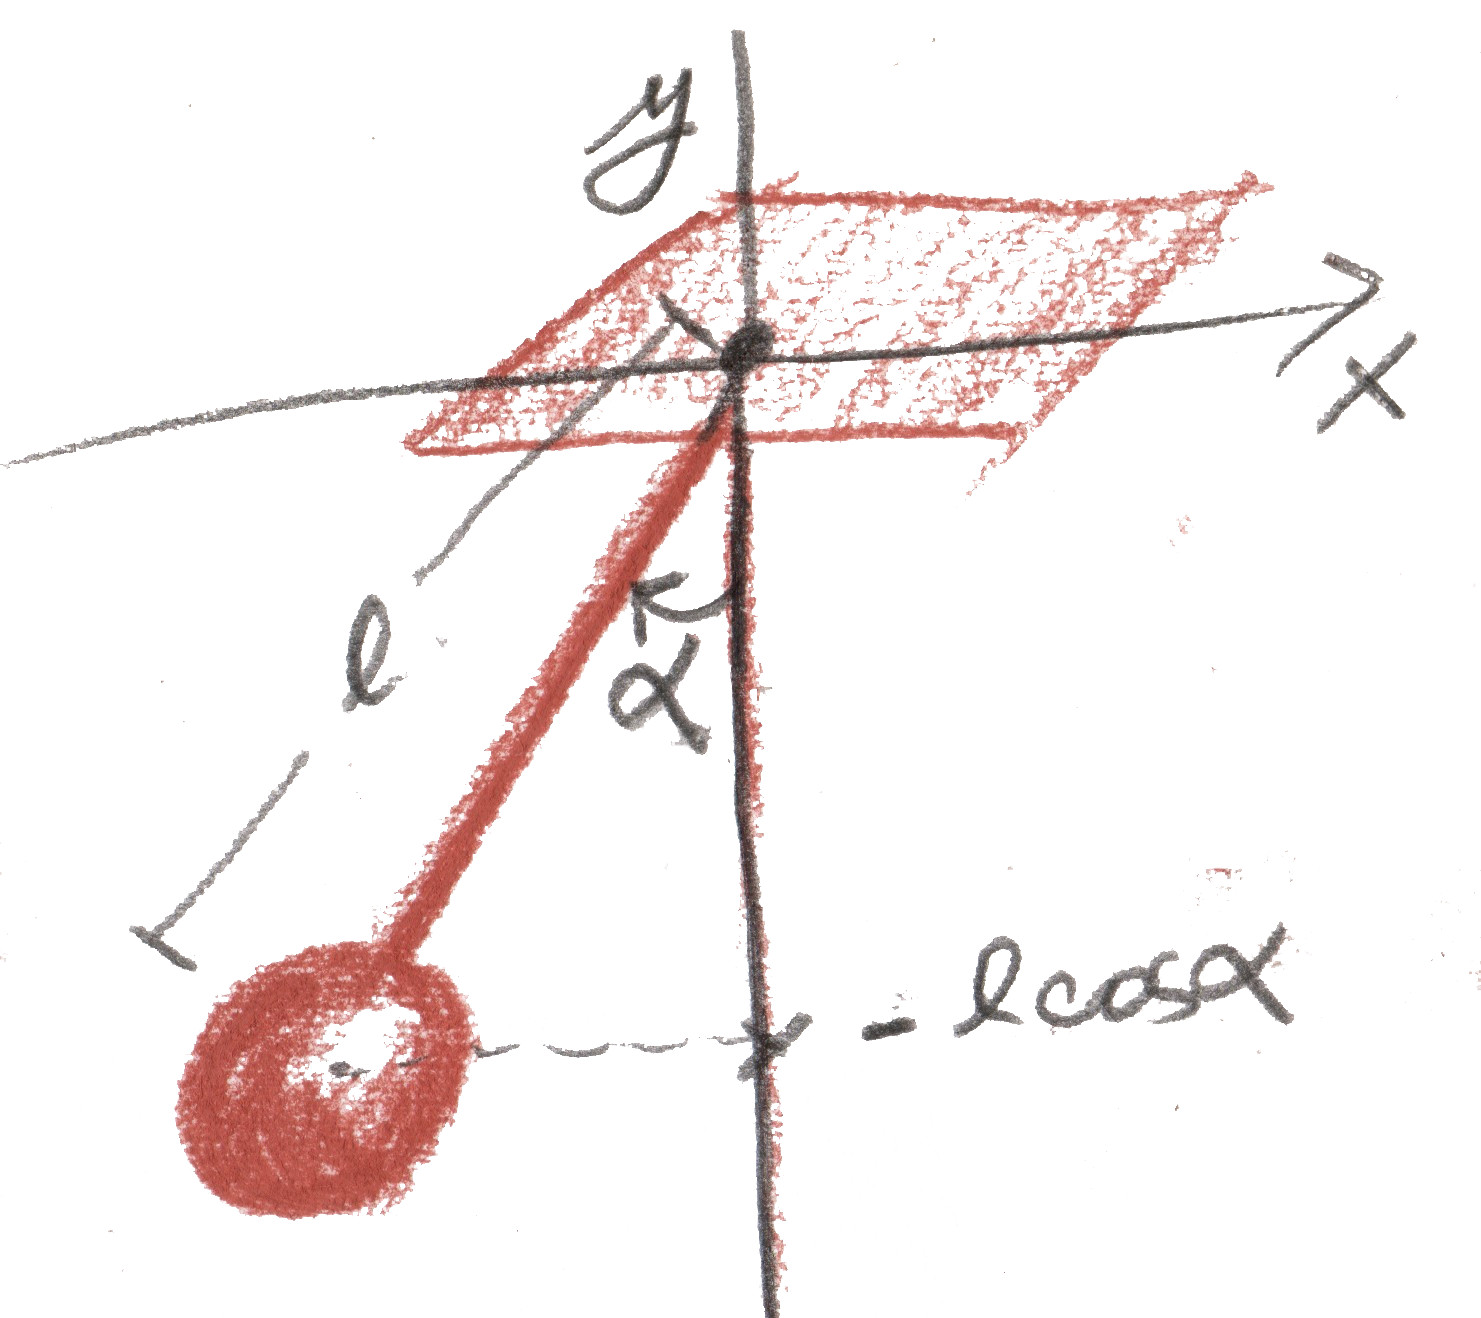
\includegraphics[scale=.07]{imagenes/pendulo.jpg} & Se trata de una masa puntual $m$ suspendida de un punto por medio de una barra de longitud $l$
 a la que suponemos sin masa. Equivale al movimiento sobre una guía circular.  Usaremos el ángulo $\alpha$ marcado en la figura, como variable dependiente.
\end{tabular}
Supondremos que el origen del sistema de de coordenadas está sobre el punto de amarre de la barra. Entonces de \eqref{cons_ener} con $t_1=t$ deducimos 
\[\begin{split}\frac{m|v(t)|^2}{2}-\frac{m|v(t_0)|^2}{2}&=-mg\left(y(t)-y(t_0)\right)\\
  &=mg\cos\alpha(t)-mg\cos\alpha(t_0).
   \end{split}
\]
\end{frame}


\begin{frame}{El péndulo}
Ahora la posición de la masa es $x(t)=l(\sen\alpha,-\cos\alpha)$ luego 
\[v(t)=l\alpha'(t)(\cos\alpha,\sen\alpha) \Longrightarrow |v(t)|^2=l^2\alpha'(t)^2.\]
Entonces
\[\frac{ml^2\alpha'(t)^2}{2}= mgl\cos\alpha(t)-mgl\cos\alpha(t_0) +\frac{mv(t_0)^2}{2}.\]
Derivando esta relación
\[ml^2\alpha'(t)\alpha''(t)=-mgl\alpha'(t)\sen\alpha(t).\]
De esto deducimos la ecuación del \href{http://es.wikipedia.org/wiki/Péndulo}{péndulo}
\[\boxed{\alpha''(t)=-\frac{g}{l}\sen\alpha(t)}.\]
\end{frame}

\begin{frame}{La braquistócrona}
 
\textbf{Problema} Dados dos puntos $A$ y $B$ en las proximidades de la superficie terrestre, uno mas abajo respecto al suelo que el otro,
queremos diseñar el tobogán óptimo entre los dos, 
esto es el tobogán que nos lleve de $A$ hasta $B$ en el menor tiempo. La curva solución a este problema se llama curva 
\href{http://es.wikipedia.org/wiki/Curva_braquistócrona}{braquistócrona} (braquistos - el más corto, cronos - tiempo). 
 
\begin{center}
\animategraphics[controls,scale=.5]{15}{braquis/braquis-}{0}{105}
\end{center}
\end{frame}

\begin{frame}{La braquistócrona}
\nl Este problema fue resuelto por primera vez por Johann Bernoulli y es quizás el problema  que abrió la rama de las matemáticas que se denomina 
\href{http://es.wikipedia.org/wiki/Cálculo_variacional}{cálculo de 
variaciones}. Vamos a dar la solución de Bernoulli que es muy elegante y está basada en un resultado de óptica llamado 
 el \href{http://es.wikipedia.org/wiki/Principio_de_Fermat}{Principio de Mínimo Tiempo} de \href{http://es.wikipedia.org/wiki/Fermat}{Fermat}.




\end{frame}


\begin{frame}{Principio de Fermat}

\nl\begin{block}{\href{http://es.wikipedia.org/wiki/Principio_de_Fermat}{Principio de Mínimo Tiempo} de \href{http://es.wikipedia.org/wiki/Fermat}{Fermat}}
 La luz sigue para ir de un punto a otro el recorrido que minimiza el tiempo.
\end{block}

\nl La primera impresión   es que ese reccorrido debería ser la línea recta. Si embargo esto no es así debido a que la velocidad de la luz cambia
de acuerdo al \href{http://es.wikipedia.org/wiki/Velocidad_de_la_luz_en_un_medio_material}{medio que atraviesa}. 
La velocidad de la luz en el vacío es 299.792,458km/h y en el diamante 124.034,943 km/h. La velocidad de la luz cambia no sólo con la sustancia sino con sus cualidades, 
como la densidad. 

\nl Si la luz se mueve dentro de un medio homogéneo, el camino que sigue es la línea recta. Las cosas cambian cuando la luz cambia de medio de propagación. Por ejemplo
cuando pasa del aire al vidrio. 

\end{frame}

\begin{frame}{Principio de Fermat}
\begin{tabular}{m{4cm} m{5.5cm}}
 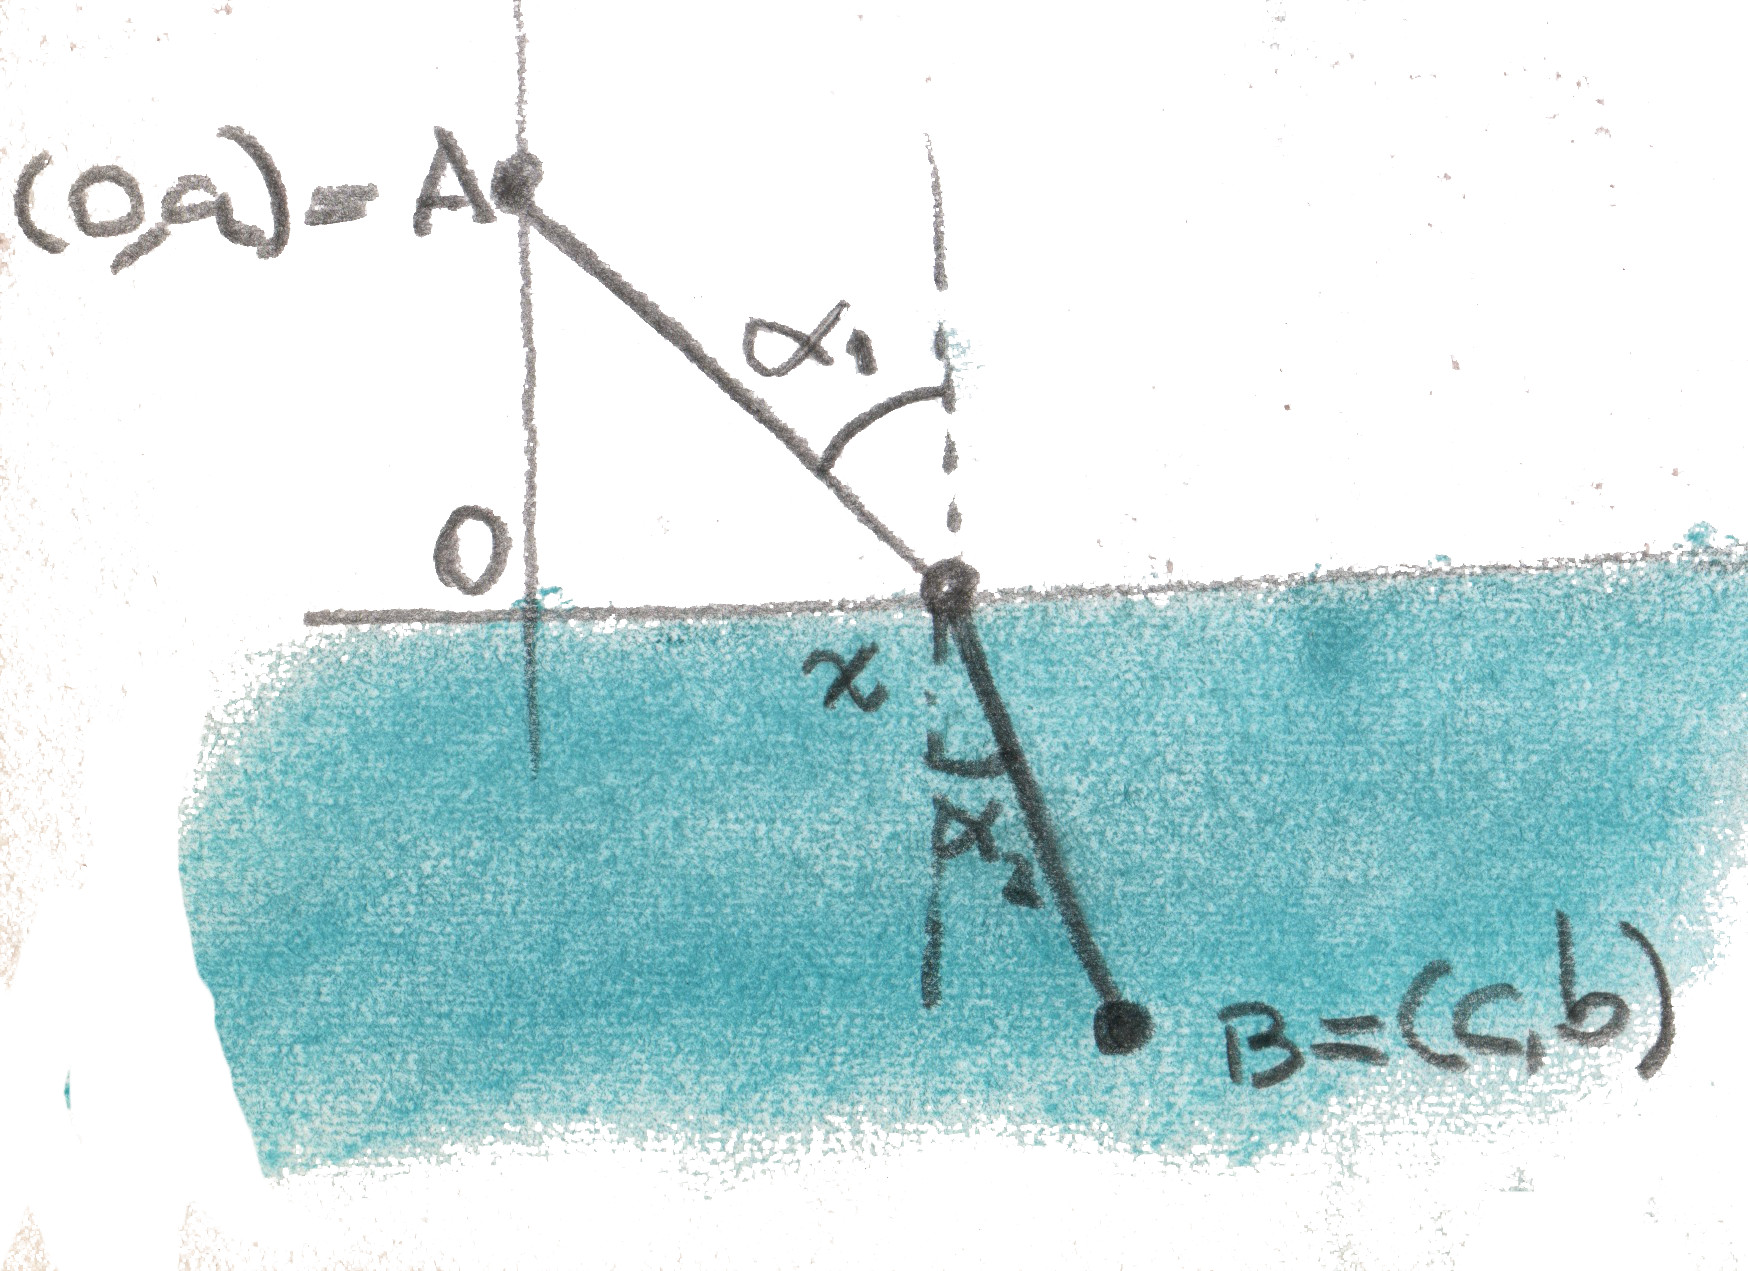
\includegraphics[scale=.07]{imagenes/refraccion.jpg} & Supongamos que la luz une los puntos $A$ y $B$ del plano y en el camino atravieza de un medio a otro, siendo la velocidad
 de la luz en cada uno de ellos $v_1$ y $v_2$. 
 \end{tabular}
Supongamos que $A=(a,0)$ y $B=(c,b)$ y el eje $x$ es la frontera entre los medios. Como sabemos que mientras se mueva en un medio homogéneo la luz sigue en línea recta, 
el tiempo que emplea la luz para ir $A$ a $B$ es
 \[t=\frac{\sqrt{a^{2} + x^{2}}}{v_{1}} + \frac{\sqrt{{\left(c - x\right)}^{2} + b^{2}}}{v_{2}}\]
 
\end{frame}

\begin{frame}{Ley de refracción de snell}
Para determinar la trayectoria es suficiente encontrar $x$, el punto donde la luz choca con la interfaz entre los medios. 
El principio de Fermat afirma que el tiempo es mínimo de modo que hallaremos un punto crítico de $t$ respecto a $x$. 
\[ \frac{dt}{dx}=-\frac{c - x}{\sqrt{{\left(c - x\right)}^{2} + b^{2}} v_{2}} +
\frac{x}{\sqrt{a^{2} + x^{2}} v_{1}}=\frac{\sen\alpha_1}{v_1}-\frac{\sen\alpha_2}{v_2} \]
Deducimos que en un punto crítico 
\[\boxed{\frac{\sen\alpha_1}{v_1}=\frac{\sen\alpha_2}{v_2} }\]
que se denomina \href{http://es.wikipedia.org/wiki/Ley_de_Snell}{Ley de Snell}. El punto crítico es mínimo pues $\left.\frac{dt}{dx}\right|_{x=0}=-\tfrac{c}{bv_2}<0$ y
$\left.\frac{dt}{dx}\right|_{x=c}=\tfrac{c}{\sqrt{c^2+a^2}v_1}>0$.

 
\end{frame}

\begin{frame}{Ley de refracción de snell}
\nl A la razón entre la velocidad de la luz dentro de un determinado medio y la velocidad de la luz en el vacio se lo denomina 
\href{http://es.wikipedia.org/wiki/Índice_de_refracción}{índice de refracción} y se lo denota con la letra $n$. La Ley de Snell se la suele escribir
\[\boxed{n_1\sen\alpha_1=n_2\sen\alpha_2 }.\]
Que pasa si la luz atraviesa un medio que va cambiando de manera continua de índice de refracción. Por ejemplo, el índice de refracción en la atmósfera
va cambiando de manera continua con la altitud respecto a la superficie terrestre, ya que la densidad del aire va cambiando con la altitud. La Ley de
Snell en este caso es
\[\boxed{\frac{\sen\alpha}{v}=\text{cte}}\]
Aquí el ángulo $\alpha$ y la velocidad $v$ cambian respecto a alguna variable/s real/es, por ejemplo la altitud.

\end{frame}


\begin{frame}{Volviendo a la braquistócrona}
\nl¿Que tienen en común el recorrido de la luz y la braquistócrona? Bernoulli se dió cuenta que la situación en los dos casos es la misma, ya que en los dos casos 
se trata de minimizar el tiempo del recorrido. De modo que la braquistócrona también tiene que satisfacer la Ley de Snell.\newline  
\nl Ahora sopongamos un sistema de coordenadas con origen en el punto $A$, inicial del recorrido, y que parte desde $A$   
del reposo. Con estas suposiciones $x(t_0)=0$ y $v(t_0)=0$. Por la conservación de la energía 
\[\frac{m}{2}|v(t)|^2=-mgy(t)=mg|y(t)|.\]
\nl Así por la ley de Snell
\[\frac{\sen\alpha}{|v(t)|}=\frac{\sen\alpha}{\sqrt{2g|y|}}=c=\text{ cte}.\]

  \end{frame}

\begin{frame}{Ecuación de la braquistócrona}
En \eqref{cos_alpha} habíamos expresado el $\cos\alpha$ (en realidad del ángulo opuesto por el vértice, pero es igual) mediante la derivada. Luego
\[\sen\alpha=\sqrt{1-\cos^2\alpha}=\frac{1}{\sqrt{1+y'(x)^2}}.\]
Entonces tenemos
\[\sqrt{2g|y|}\sqrt{1+y'(x)^2}=c=\hbox{ cte}\]
Despejando llegamos a la ecuación diferencial
\[\boxed{\sqrt{\frac{y}{c-y}}y'=1}.\]
Es una ecuación con variables separables. La constante $c$ no tiene el mismo valor que en la ecuación anterior.  
  \end{frame}

  \begin{frame}{Resolviendo la ecuación de la braquistócrona}
La solución se obtiene resolviendo
\[x=\int dx=\int \sqrt{\frac{y}{c-y}}dy.\]
Hacemos el cambio de variables
\[\sqrt{\frac{y}{c-y}}=\tan\phi\Longrightarrow y=c\sen^2\phi\Longrightarrow dy=2c\sen\phi\cos\phi d\phi.\]
Luego
\[x=2c\int\sen^2\phi d\phi=\frac{c}{2}\left(2\phi-\sen 2\phi\right)+C_1.\]
Como tiene que pasar por $x=0$ e $y=0$ debe ser $C_1=0$

  \end{frame}

  \begin{frame}{La cicloide}
 Tenemos que
 \[\left\{\begin{array}{l l l}
	      y&=c\sen^2 \phi&=\frac{c}{2}(1-\cos2\phi)\\
	      x&=\frac{c}{2}(2\phi-\sen2\phi)\ &\\
          \end{array}\right.
\]
Conviene llamar $2\phi=\theta$ y $a=c/2$
 \[\left\{\begin{array}{l l }
	      y&= a(1-\cos\theta)\\
	      x&=a(\theta-\sen\theta)\
          \end{array}\right.
\]
Que son la ecuaciones paramétricas de una curva conocida con el nombre de \href{http://es.wikipedia.org/wiki/Cicloide}{cicloide}. Ver el enlace anterior para ver 
otras propiedades notables de esta curva.
\begin{center}
\animategraphics[controls,scale=.5]{15}{cicloide/cicloide-}{0}{31}
\end{center}
  
  \end{frame}


  \begin{frame}{La tautócrona}
  Vamos a ver otra propiedad notable de la ciclode. Supongamos que dejamos caer el cuerpo del reposo desde un punto intermedio, digamos en $(x_0,y_0)$. Sea  $\theta_0$
 el valor del paŕámetro $\theta$ correpondiente a este punto. ¿Cuánto tardara en llegar el cuerpo al punto mínimo de la curva que ocurre cuando $\theta=\pi$? 
\begin{center}
\animategraphics[controls,scale=.5]{15}{tautocrona/tauto-}{0}{79}
\end{center}

  \end{frame}
  
  
  \begin{frame}{La tautócrona}
\nl Tenemos
\[
 \left\{ \begin{array}{l l}
 \frac{dx}{d\theta}&=a(1-\cos\theta)\\
 \frac{dy}{d\theta}&=a\sen\theta 
 \end{array}\right.
\]
% 
Como el cuerpo ahora no parte de $(0,0)$ tendremos
\[|v|=\sqrt{2g(y_0-y)}.\]

  \end{frame}
  
  \begin{frame}{La tautócrona}
Por \eqref{2ley} $ds/dt=|v|$. Si llamamos $T$ al tiempo que demanda en llegar a $\theta=\pi$, y llamamos  $s_0$ y $s_1$ a los arcos correspondientes al punto inicial
y final.  Tenemos
 \[T=\int_0^Tdt=\int_{s_0}^{s_1}\frac{dt}{ds}ds=\int_{s_0}^{s_1}\frac{1}{\sqrt{2g(y_0-y)}}ds.\]
 
Cambiando la variable de integración a $\theta$. Como 
\[
 \frac{ds}{d\theta}=\sqrt{\left(\frac{dx}{d\theta}\right)^2+\left(\frac{dy}{d\theta}\right)^2}=\sqrt{2}a\sqrt{1-cos\theta}.
\]
 Tenemos

  \end{frame}
   \begin{frame}{La tautócrona}

\[T=\sqrt{\frac{a}{g}}\int_{\theta_0}^{\pi}\frac{\sqrt{1-\cos\theta}}{\cos\theta_0-\cos\theta}d\theta=
\sqrt{\frac{a}{g}}\int_{\theta_0}^{\pi}\frac{\sen\frac{\theta}{2}}{\cos^2\frac{\theta_0}{2}-\cos^2\frac{\theta}{2}}d\theta.
\]
Ahora hacemos la sustitución
\[u=\frac{\cos\frac{\theta}{2}}{\cos\frac{\theta_0}{2}}\Longrightarrow du=-\frac{\sen\frac{\theta}{2}}{2\cos\frac{\theta_0}{2}}d\theta.\]
Y vemos que
\[
 T=2\sqrt{\frac{a}{g}}\int_0^1\frac{1}{\sqrt{1-u^2}}du.
\]
Que es una expresión independiente de $\theta_0$. En consecuencia el tiempo $T$ que demanda  el cuerpo para llegar $\theta=\pi$ es siempre el mismo no importa
desde donde se deje caer.
  \end{frame} 

\end{document}